\documentclass{article}[12pt]
\setlength{\textheight}{8.75in}
\setlength{\topmargin}{-0.5in}
\setlength{\oddsidemargin}{-.25in}
\setlength{\evensidemargin}{0in}
\setlength{\textwidth}{7in}
\usepackage{amsfonts, amsmath, amsthm, amssymb, mathrsfs, graphicx, fancyhdr, cancel, latexsym, multicol, setspace}

%\usepackage{savesym}
%\usepackage{amsmath}
%\savesymbol{iint}
%\usepackage{txfonts}
%\restoresymbol{TXF}{iint}

\pagestyle{fancy}
\lhead{Jonathan McFadden \\ Spring 2019}
\rhead{TCSS 551 \\ Term Project}
\headsep = 22pt 
\headheight = 15pt


\doublespacing

% BEGIN PRE-AMBLE


% Setup equation numbering 
\numberwithin{equation}{subsection} 

%Equation Numbering Shortcut Commands
\newcommand{\numbch}[1]{\setcounter{section}{#1} \setcounter{equation}{0}}
\newcommand{\numbpr}[1]{\setcounter{subsection}{#1} \setcounter{equation}{0}}
\newcommand{\note}{\textbf{NOTE:  }}

%Formatting shortcut commands
\newcommand{\chap}[1]{\begin{center}\begin{Large}\textbf{\underline{#1}}\end{Large}\end{center}}
\newcommand{\prob}[1]{\textbf{\underline{Problem #1):}}}
\newcommand{\sol}[1]{\textbf{\underline{Solution #1):}}}
\newcommand{\MMA}{\emph{Mathematica }}

%Text Shortcut Command
\newcommand{\s}[1]{\emph{Side #1}}

% Math shortcut commands
\newcommand{\pd}[2]{\frac{\partial #1}{\partial #2}}
\newcommand{\pdn}[3]{\frac{\partial^{#1} #2}{\partial #3^{#1}}}
\newcommand{\infint}{\int_{-\infty}^\infty}
\newcommand{\infiint}{\iint_{-\infty}^\infty}
\newcommand{\infiiint}{\iiint_{-\infty}^\infty}
\newcommand{\dint}[2]{\int_{#1}^{#2}}
\newcommand{\dd}[1]{\textrm{d#1}}
\newcommand{\ddd}[1]{\textrm{d}#1}
\renewcommand{\Re}{\mathbb{R}}

%Math Text
\newcommand{\csch}{\text{ csch}}

%Physics Shortcut Commands
\newcommand{\h}{\mathcal{H}}
\newcommand{\Z}{\mathcal{Z}}


% END PRE-AMBLE




\begin{document}

\begin{center}
\begin{Large} \textbf{\underline{Forest Cover Analysis}} \end{Large}
\end{center}

\begin{center}
\begin{large} \emph{TCSS-551 Term Project} \end{large}
\end{center}

\begin{center} Jonathan McFadden \end{center}


\vspace{2.75in}



\begin{flushleft}


\begin{large} \textbf{\underline{Introduction}} \end{large}

The goal of this project is twofold.  First, we seek to create an accurate big-data/machine-learning model to predict which type of trees will grow best in a certain area based on the conditions of that area.  Finally, we seek to determine which features of a given area are most important for determine which type of tree will grow best there.  To do this, we have chosen three different methods:

\begin{itemize}
\item Linear/Logistic Regression
\item Decision Trees
\item Random Forest
\end{itemize}

We chose to try a Linear/Logistic regression first because they're provide a simple and low computational cost way to see a relationship between the features and outcomes of the provided data does indeed exist.  This method will be unlikely produce predictions with good accuracy due to its simplicity, however should these methods show a relationship or relationships within the provided data, that would be a positive indicator to proceed to more complicated and compute intensive algorithms.


\vspace{1.25in}

\begin{large} \textbf{\underline{METHOD A} - Linear/Logistic Regression} \end{large}

As described above, the initial method we tried were Linear/Logistic Regressions.  We tried three variations on this method.  First, we ran a simple linear regression.  This gave a poor result, but \emph{did} indicate that there was a relation between the features and outcomes in the data.  This linear model gave an $R^2$ value of $0.4214$ on the test data and $0.4006$ on the training data.  This is odd as, one would expect this value to be higher for the training data than the test data.  This trend also continued when comparing via MSE\footnote{mean squared error}, as the training data had an MSE of $2.3952$ while the test data had an MSE of $2.3257$.  \newline

We followed this basic Linear Regression model with two Logistic Regression models; one based on fitting a binary problem for each class (\emph{OVR}) and the other based on a multinomial fitting (\emph{MULTNOM}).  The \emph{OVR} Logistic Regression had a mean error of $0.6711$ and an MSE of $2.8735$ on the test data.  The \emph{MULTNOM} Logistic Regression did slightly better on mean error with $0.6653$ and slightly worse on the MSE with $3.2866$ on the test data.  Interestingly, the \emph{OVR} Logistic Regression had a better MSE on the test data than on the training data ($2.9991$) while the \emph{MULTNOM} Logistic Regression had a better mean error on the test data than the training data ($0.6721$). \newline

While this method did establish that \emph{there is} a relationship between the features and outcomes in the data, it does not have very good accuracy.  More importantly, it does not tell us anything about which features are most important for determining which type of tree will do best in a certain area.  However, now that we know there is a relationship within the data, we can move on to more complicated and computationally intense methods to determine the importance of the various features.


\vspace{1.25in}

\begin{large} \textbf{\underline{METHOD B} - Decision Trees} \end{large}

The first detailed method we chose to use was Decision Trees.  We chose to use this method because it is relatively simple\footnote{as far as ML algorithms go}, yet very powerful as it has the ability to give us an idea of which features are most important.  To determine feature importance, we built three different decision trees, with 3, 4, and 5 levels respectively.  These decision tress can be graphically represented as

\end{flushleft}

\begin{center}
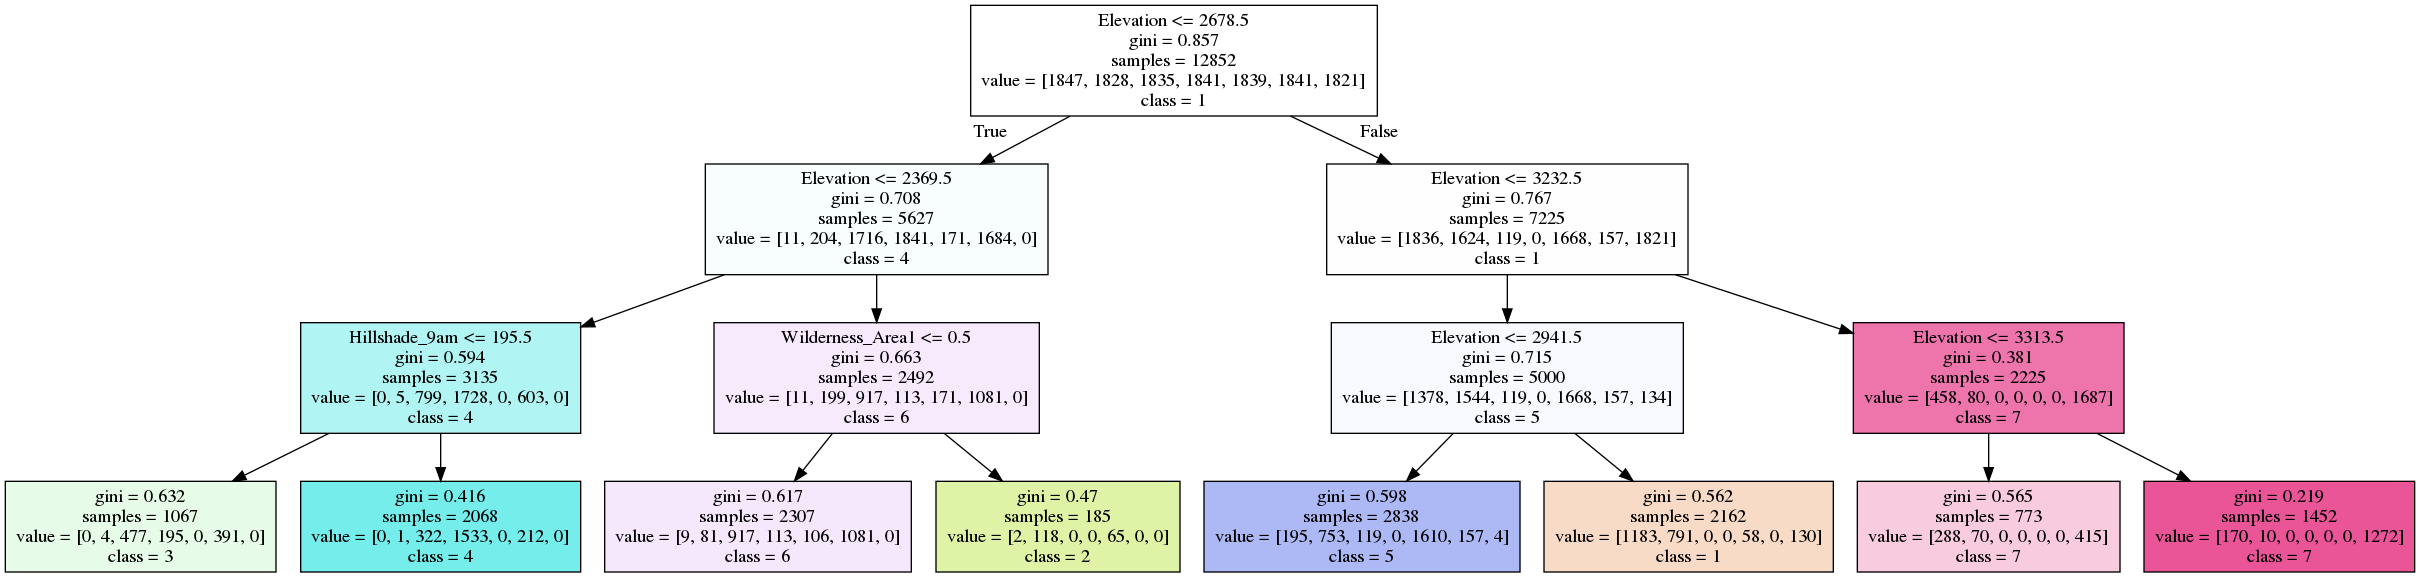
\includegraphics[width=7in]{../decTree1.png}
\end{center}

\begin{center}
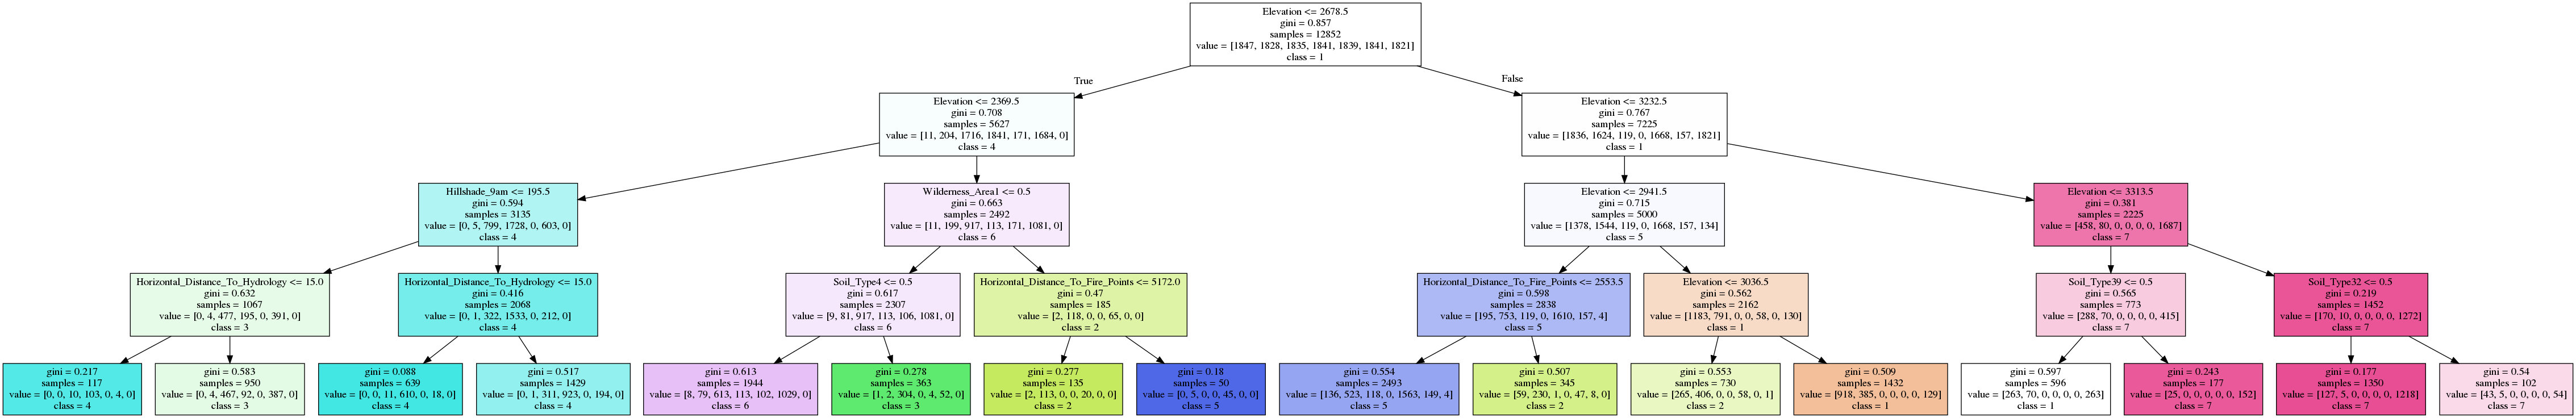
\includegraphics[width=7in]{../decTree2.png}
\end{center}

\begin{center}
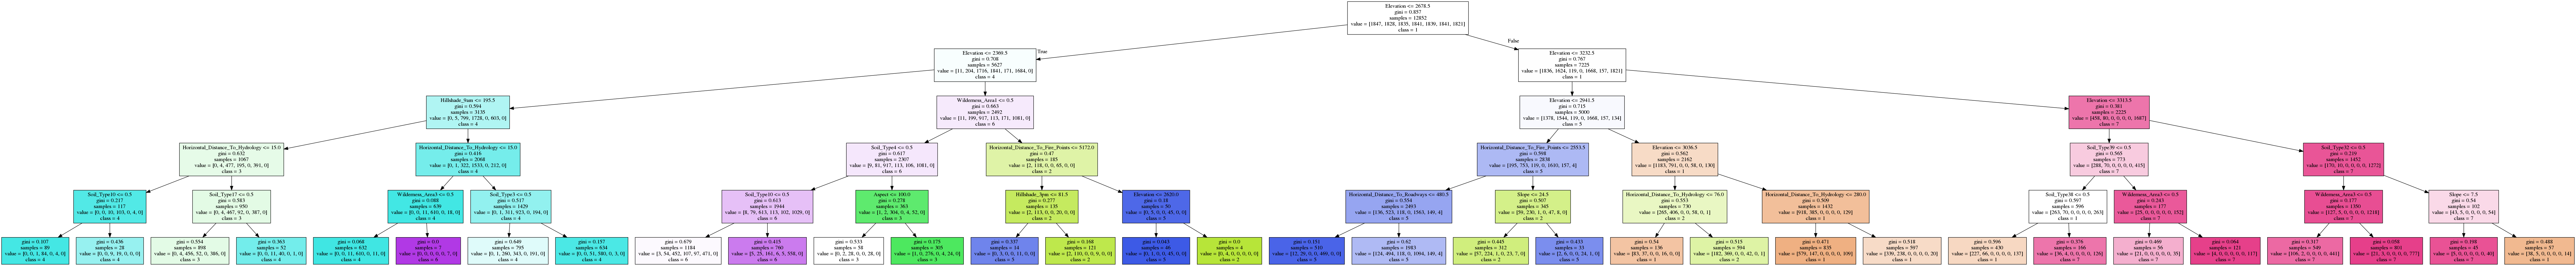
\includegraphics[width=7in]{../decTree3.png}
\end{center}
\begin{flushleft}


From these trees, we can clearly see that \textbf{Elevation} is the most important determining feature, by far.  We can also see that \textbf{Elevation} is flowed by, in no particular order, the features:

\begin{itemize}
\item \textbf{Horizontal Distance To Fire Points}
\item \textbf{Horizontal Distance To Hydrology}
\item \textbf{Hillside Shade 9am}
\item \textbf{Wildernes Area 1}
\item \textbf{Soil Type4}
\end{itemize}

For the last part of applying the Decision Tree algorithm to this data, we constructed a Decision Tree with no limit on its depth to use for making predictions.  This complete Decision Tree model has a mean accuracy of $0.8078$ and an MSE of $1.7571$, beating the Linear/Logistic Regression by a \emph{large} margin.


\vspace{1.5in}

\begin{large} \textbf{\underline{METHOD C} - Random Forest} \end{large}

The last model we applied to this problem was a Random Forest model.  Since the Decision Tree model worked well, the natural extension was a Random Forest.  As an ensemble model, Random Forests can be far more powerful than Decision Trees and can give a fairly definitive (\emph{and quantified}) answer regarding which features are most important.  Running this model with 10,000 trees, we had a mean accuracy of $0.8748$ and an MSE of $1.0044$, beating the previously superior Decision Tree model by almost 50\%.  More importantly, we found that the top 15 features were:

\begin{itemize}
\item \textbf{Elevation} : 0.2264
\item \textbf{Horizontal Distance to roadways} : 0.0918
\item \textbf{Horizontal Distance to fire points} : 0.0728
\item \textbf{Horizontal Distance to Hydrology} : 0.0631
\item \textbf{Vertical Distance to Hydrology} : 0.0539
\item \textbf{Hillshade Shade 9am} : 0.0518
\item \textbf{Aspect} : 0.0499
\item \textbf{Hillshade 3pm} : 0.0468
\item \textbf{Hillshade Noon} : 0.0450
\item \textbf{Wilderness Area4} : 0.0434
\item \textbf{Slope} : 0.0366
\item \textbf{Soil Type10} : 0.0230
\item \textbf{Soil Type38} : 0.0191
\item \textbf{Wilderness Area 1} : 0.0187
\item \textbf{Soil Type3} : 0.0186
\end{itemize}

This allows to determine the relative importances of features so that we can better understand what features affect the success or failure of different tree species in various areas.  Additionally, should we wish to create an even more powerful predictive model (\emph{i.e. a neural network}) these importances can tell us which features we should include in the network and which we can discard or combine as a way to reduce the computational complexity of training the network.  \newline

By graphing the feature importances sorted from largest to smallest, we see that there are two "cliffs" where feature importances suddenly drop, one following 10 (\emph{Wilderness Area4}) and one following 12 (\emph{Soil Type10}).  To see this better, we graph the Random Forest Feature Importances 

\end{flushleft}

\begin{center}
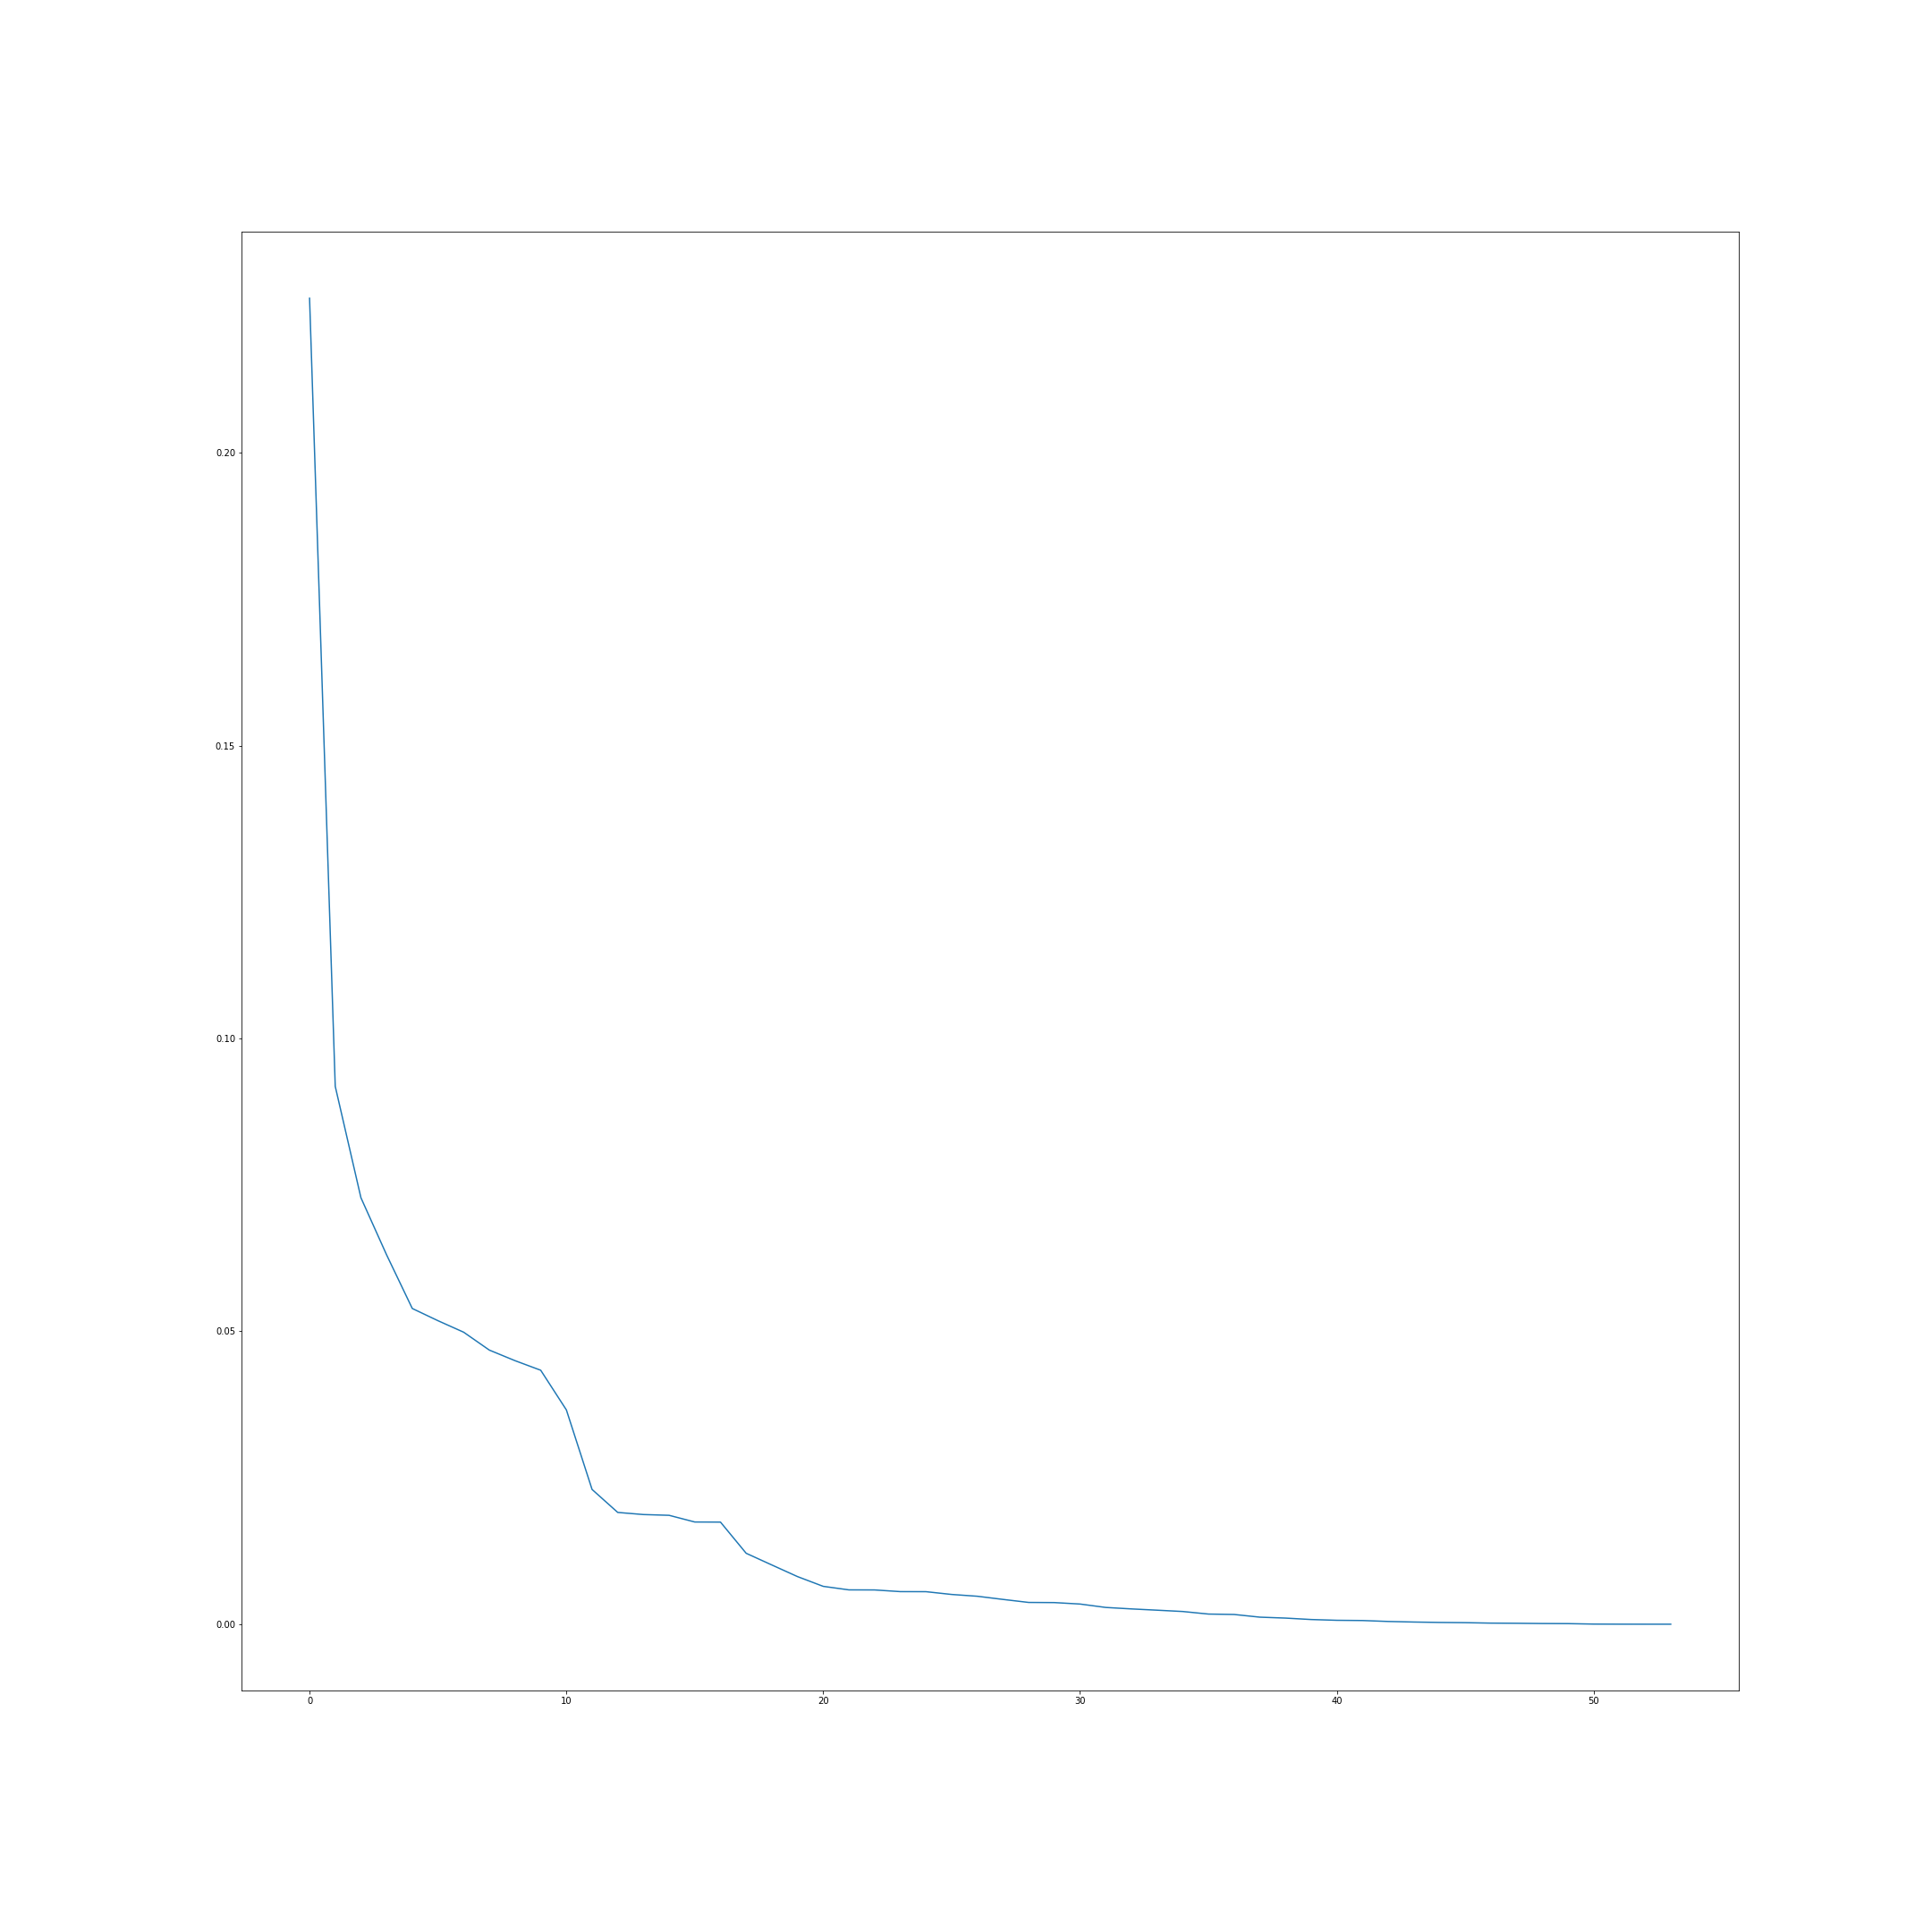
\includegraphics[width=5in]{../randForImpt.png}
\end{center}

\begin{flushleft}

This indicates that we could truncate at the 10 most important features or the 12 most important features.  However, running this through a Singular Value Decomposition as a verification on the Random Forest Feature Importances, we get the graph of the Singular Values

\end{flushleft}

\begin{center}
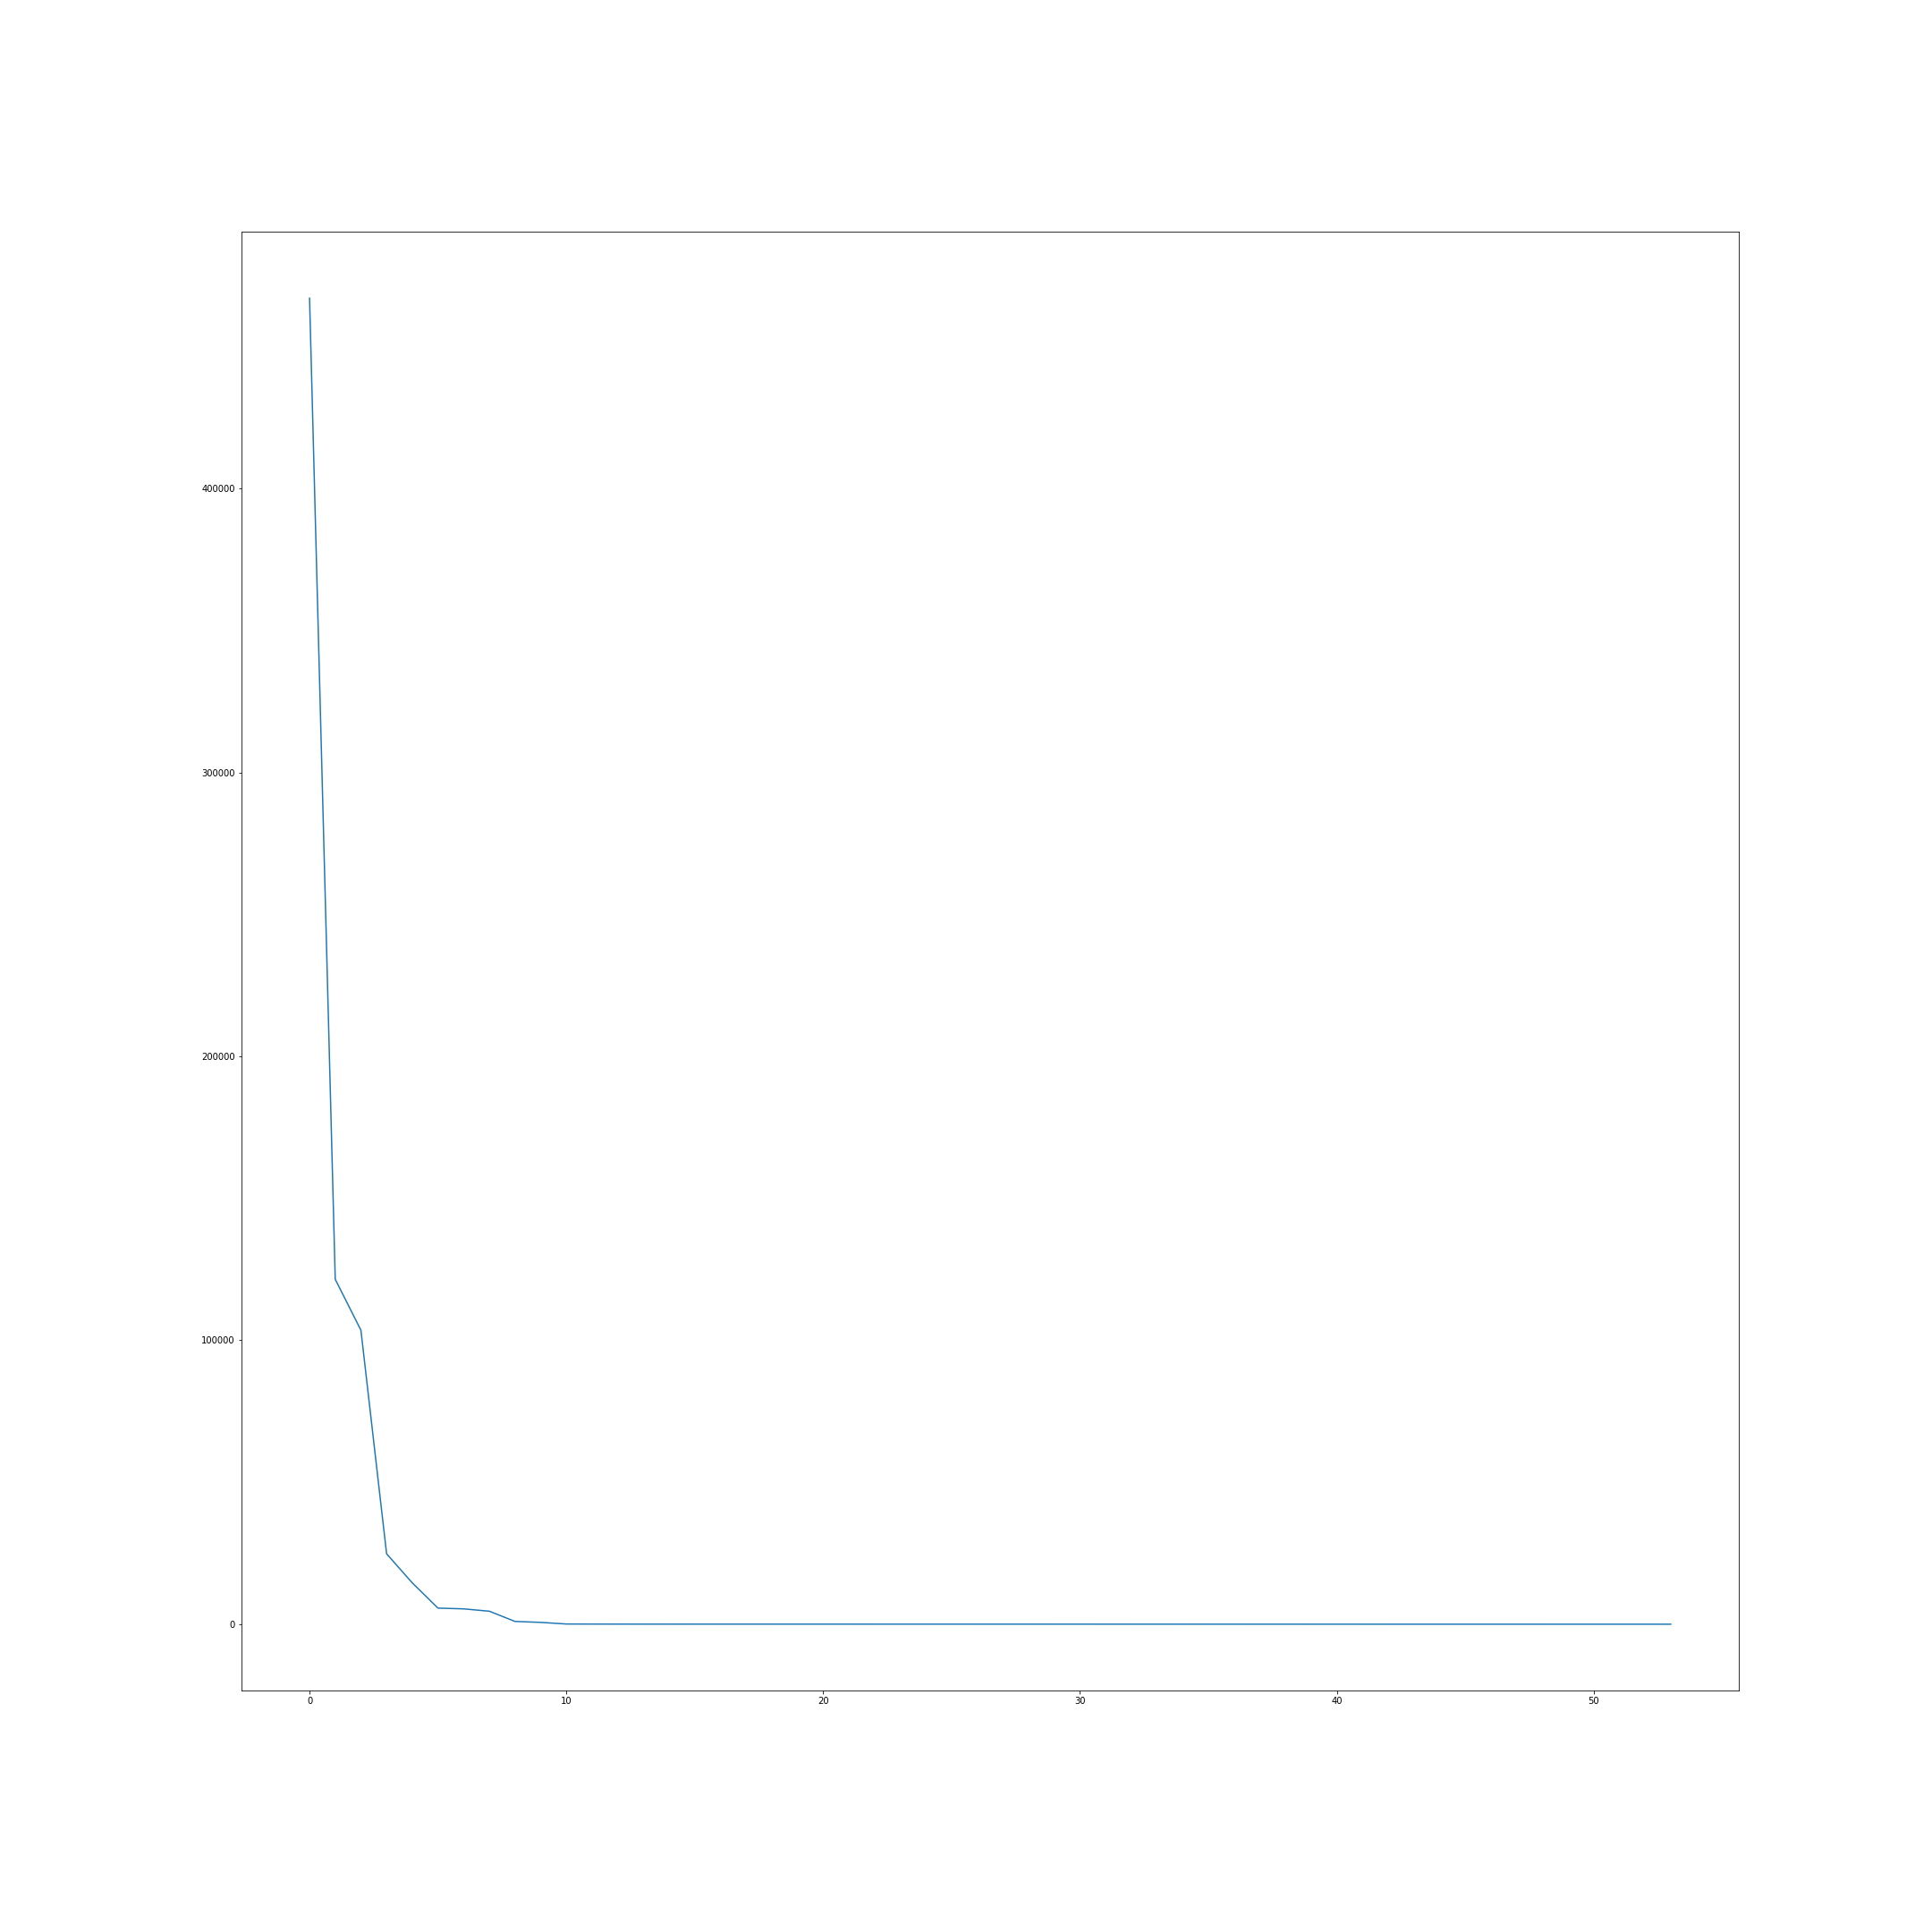
\includegraphics[width=5in]{../SVDimport.png}
\end{center}

\begin{flushleft}
\emph{This} plot indicates that truncating after the first ten features is best as the second "cliff" following 12, appears to be an artifact from the approximate nature of the Random Forest algorithm, although we only know this because the dataset if small enough to reasonable compute the singular values.  This plot of the singular values also indicates that we could also truncate after the fifth or sixth most important features, but, again, this is only apparent because we \emph{can} compute a SVD for this data.


\vspace{1.5in}

\begin{large} \textbf{\underline{Results}} \end{large}

Numerical results are contained within the explanation for each algorithm, however we can summarize them by stating that

\begin{quote}
Linear/Logistic Regressions provided relatively poor predictions and no information on feature importances, but did indicate the presence of a relationship within the data.  Decision Trees far outperformed Linear/Logistic Regressions.  Additionally, Decision Trees also told us that elevation was the most important feature, but could not quantify this.  Random Forests not only improved on the predictions of Decision Trees by 50\%.  Moreover, the Random Forest also quantified feature importances with good accuracy compared to a Singular Value Decomposition, but with much less computation cost than a SVD.
\end{quote}

Based on this, running an entropic method like Decision Trees or an ensemble method like a Random Forest are  powerful and relatively simple ways to analyze large datasets.


































































\end{flushleft}

\end{document}
